\documentclass[11pt,a4paper,twoside]{report}

% ============================================================================
% PACKAGES
% ============================================================================

% Page geometry and layout
\usepackage[
    top=1in,
    bottom=1.25in,
    left=1.25in,
    right=1in,
    headheight=14pt
]{geometry}

% Typography and fonts
\usepackage[T1]{fontenc}
\usepackage{setspace}

% Language and encoding
\usepackage[utf8]{inputenc}
\usepackage[english]{babel}

% Colors and graphics
\usepackage[dvipsnames,svgnames,table]{xcolor}
\usepackage{graphicx}
\usepackage{tikz}
\usetikzlibrary{shapes,arrows,positioning,calc,shadows,decorations.pathmorphing}

% Tables and lists
\usepackage{booktabs}
\usepackage{longtable}
\usepackage{tabularx}
\usepackage{multirow}
\usepackage{enumitem}

% Headers and footers
\usepackage{fancyhdr}
\usepackage{titlesec}
\usepackage{titletoc}

% Cross-references and hyperlinks
\usepackage[
    colorlinks=true,
    linkcolor=NavyBlue,
    citecolor=ForestGreen,
    urlcolor=RoyalBlue,
    bookmarks=true,
    bookmarksnumbered=true,
    pdfstartview=FitH
]{hyperref}
\usepackage{bookmark}

% Math and symbols
\usepackage{amsmath}
\usepackage{amssymb}
\usepackage{siunitx}

% Boxes and callouts
\usepackage{tcolorbox}
\tcbuselibrary{skins,breakable}

% Code listings (for any code snippets)
\usepackage{listings}

% Miscellaneous
\usepackage{lipsum}
\usepackage{parskip}
\usepackage{float}
\usepackage{subcaption}

% ============================================================================
% COLOR DEFINITIONS
% ============================================================================

\definecolor{chaptercolor}{RGB}{0,82,147}
\definecolor{sectioncolor}{RGB}{0,102,179}
\definecolor{phasecolor1}{RGB}{46,139,87}    % SeaGreen
\definecolor{phasecolor2}{RGB}{70,130,180}   % SteelBlue  
\definecolor{phasecolor3}{RGB}{148,103,189}  % Purple
\definecolor{projectbg}{RGB}{245,248,250}
\definecolor{skillsbg}{RGB}{255,250,240}
\definecolor{suggestionbg}{RGB}{240,255,240}
\definecolor{warningbg}{RGB}{255,248,220}
\definecolor{codebg}{RGB}{248,248,248}

% ============================================================================
% TCOLORBOX STYLES
% ============================================================================

\newtcolorbox{projectbox}[2][]{
    enhanced,
    colback=projectbg,
    colframe=sectioncolor,
    fonttitle=\bfseries\large,
    title={#2},
    attach boxed title to top left={yshift=-3mm,xshift=5mm},
    boxed title style={colback=sectioncolor,colframe=sectioncolor},
    breakable,
    left=8pt,
    right=8pt,
    top=8pt,
    bottom=8pt,
    #1
}

\newtcolorbox{skillsbox}{
    enhanced,
    colback=skillsbg,
    colframe=orange!60!black,
    fonttitle=\bfseries,
    title={Key X-Chapters Skills Exercised},
    attach boxed title to top left={yshift=-2mm,xshift=4mm},
    boxed title style={colback=orange!60!black,colframe=orange!60!black},
    left=6pt,
    right=6pt,
    top=6pt,
    bottom=6pt,
}

\newtcolorbox{suggestionbox}{
    enhanced,
    colback=suggestionbg,
    colframe=ForestGreen!70!black,
    fonttitle=\bfseries,
    title={Implementation Suggestions},
    attach boxed title to top left={yshift=-2mm,xshift=4mm},
    boxed title style={colback=ForestGreen!70!black,colframe=ForestGreen!70!black},
    left=6pt,
    right=6pt,
    top=6pt,
    bottom=6pt,
}

\newtcolorbox{checklistbox}[1][]{
    enhanced,
    colback=warningbg,
    colframe=Goldenrod,
    fonttitle=\bfseries,
    title={Pre-Flight Checklist},
    attach boxed title to top left={yshift=-2mm,xshift=4mm},
    boxed title style={colback=Goldenrod,colframe=Goldenrod},
    left=6pt,
    right=6pt,
    top=6pt,
    bottom=6pt,
    #1
}

\newtcolorbox{phasebox}[2][phasecolor1]{
    enhanced,
    colback=white,
    colframe=#1,
    fonttitle=\bfseries\Large,
    title={#2},
    boxrule=2pt,
    arc=4pt,
    left=10pt,
    right=10pt,
    top=10pt,
    bottom=10pt,
    before skip=15pt,
    after skip=15pt,
    shadow={2pt}{-2pt}{0pt}{black!30},
}

% ============================================================================
% TITLE FORMATTING
% ============================================================================

\titleformat{\chapter}[display]
    {\normalfont\Huge\bfseries\color{chaptercolor}}
    {\chaptertitlename\ \thechapter}
    {20pt}
    {\Huge}
\titlespacing*{\chapter}{0pt}{-20pt}{40pt}

\titleformat{\section}
    {\normalfont\Large\bfseries\color{sectioncolor}}
    {\thesection}
    {1em}
    {}
\titlespacing*{\section}{0pt}{3.5ex plus 1ex minus .2ex}{2.3ex plus .2ex}

\titleformat{\subsection}
    {\normalfont\large\bfseries\color{sectioncolor!80!black}}
    {\thesubsection}
    {1em}
    {}

% ============================================================================
% HEADER/FOOTER SETUP
% ============================================================================

\pagestyle{fancy}
\fancyhf{}
\fancyhead[LE]{\leftmark}
\fancyhead[RO]{\rightmark}
\fancyfoot[C]{\thepage}
\renewcommand{\headrulewidth}{0.4pt}
\renewcommand{\footrulewidth}{0pt}

\fancypagestyle{plain}{
    \fancyhf{}
    \fancyfoot[C]{\thepage}
    \renewcommand{\headrulewidth}{0pt}
}

% ============================================================================
% CUSTOM COMMANDS
% ============================================================================

\newcommand{\projecttitle}[1]{\textbf{\textcolor{sectioncolor}{#1}}}
\newcommand{\skill}[1]{\textit{#1}}
\newcommand{\bookreference}[1]{\textcolor{ForestGreen}{\textbf{#1}}}

% ============================================================================
% DOCUMENT PROPERTIES
% ============================================================================

\title{%
    \vspace{-1cm}
    \rule{\textwidth}{1.5pt}\\[0.5cm]
    {\Huge\bfseries Post--X Chapters Laboratory Course}\\[0.3cm]
    {\Large\itshape A Comprehensive Project-Based Curriculum for\\
    Advanced Electronics Design}\\[0.3cm]
    \rule{\textwidth}{1.5pt}
}
\author{%
    \large Based on\\[0.2cm]
    \Large\textit{The Art of Electronics: The X Chapters}\\[0.2cm]
    \large by Paul Horowitz and Winfield Hill
}
\date{\vspace{0.5cm}\large\today}

% ============================================================================
% BEGIN DOCUMENT
% ============================================================================

\begin{document}

% ----------------------------------------------------------------------------
% TITLE PAGE
% ----------------------------------------------------------------------------

\begin{titlepage}
    \centering
    \vspace*{1cm}
    
    \begin{tikzpicture}[remember picture, overlay]
        \fill[chaptercolor!10] (current page.south west) rectangle (current page.north east);
        \draw[chaptercolor, line width=3pt] 
            ([xshift=1cm,yshift=-1cm]current page.north west) --
            ([xshift=-1cm,yshift=-1cm]current page.north east);
        \draw[chaptercolor, line width=3pt] 
            ([xshift=1cm,yshift=1cm]current page.south west) --
            ([xshift=-1cm,yshift=1cm]current page.south east);
    \end{tikzpicture}
    
    \vspace{1cm}
    
    {\fontsize{12}{14}\selectfont\textsc{A Self-Guided Laboratory Curriculum}}
    
    \vspace{1.5cm}
    
    \rule{\textwidth}{2pt}\\[0.6cm]
    {\fontsize{36}{42}\selectfont\bfseries Post--X Chapters\\Laboratory Course}\\[0.4cm]
    \rule{\textwidth}{2pt}
    
    \vspace{1cm}
    
    {\Large\itshape A Comprehensive Project-Based Approach to\\[0.2cm]
    Advanced Analog, Digital, and Embedded Systems Design}
    
    \vspace{2cm}
    
    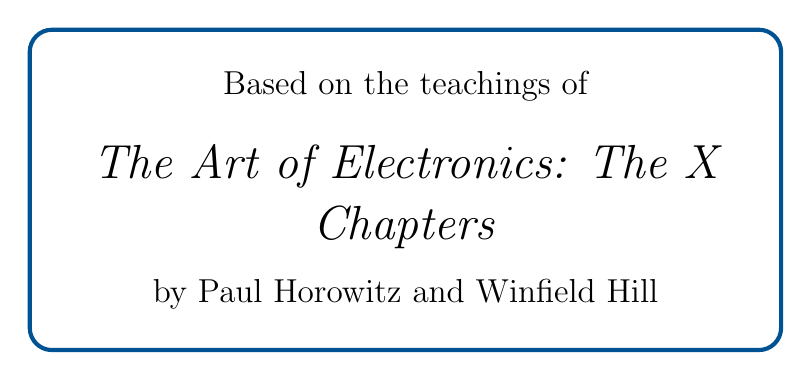
\begin{tikzpicture}
        \node[draw=chaptercolor, line width=1.5pt, rounded corners=8pt, 
              inner sep=15pt, fill=white] {
            \begin{minipage}{0.7\textwidth}
                \centering
                \large Based on the teachings of\\[0.3cm]
                \LARGE\textit{The Art of Electronics: The X Chapters}\\[0.3cm]
                \large by Paul Horowitz and Winfield Hill
            \end{minipage}
        };
    \end{tikzpicture}
    
    \vfill
    
    {\large\textsc{Curriculum Guide \& Project Roadmap}}
    
    \vspace{0.5cm}
    
    {\Large\today}
    
\end{titlepage}

% ----------------------------------------------------------------------------
% COPYRIGHT/DISCLAIMER PAGE
% ----------------------------------------------------------------------------

\thispagestyle{empty}
\vspace*{\fill}

\begin{center}
\begin{minipage}{0.8\textwidth}
\small
\textbf{About This Document}

This curriculum guide is designed to complement \textit{The Art of Electronics: The X Chapters} by providing a structured, project-based approach to mastering advanced electronics concepts. The projects herein are organized as progressive ``boss fights'' that demonstrate mastery of the skills taught in the book.

\vspace{1em}

\textbf{Prerequisites}

This curriculum assumes familiarity with basic electronics concepts as covered in the main volume of \textit{The Art of Electronics}. Students should be comfortable with fundamental circuit analysis, basic op-amp configurations, digital logic principles, and have some experience with laboratory equipment and PCB design.

\vspace{1em}

\textbf{Safety Notice}

Several projects in this curriculum involve high voltages, high currents, and potentially hazardous conditions. Always follow proper safety protocols, use appropriate protective equipment, and work within your skill level. When in doubt, seek guidance from experienced practitioners.

\vspace{1em}

\textbf{Document Version}

Version 1.0 --- \today
\end{minipage}
\end{center}

\vspace*{\fill}
\clearpage

% ----------------------------------------------------------------------------
% TABLE OF CONTENTS
% ----------------------------------------------------------------------------

\tableofcontents
\clearpage

% ----------------------------------------------------------------------------
% LIST OF PROJECTS
% ----------------------------------------------------------------------------

\chapter*{List of Projects}
\addcontentsline{toc}{chapter}{List of Projects}

\begin{longtable}{@{}p{1.5cm}p{5cm}p{2.5cm}p{4cm}@{}}
\toprule
\textbf{ID} & \textbf{Project Title} & \textbf{Phase} & \textbf{Primary Focus} \\
\midrule
\endhead

A1 & Multi-Output Lab Power Supply & Phase 1 & Power Electronics \\
A2 & Precision Transresistance Amplifier & Phase 1 & Low-Noise Analog \\
A3 & High-Speed Op-Amp Circuit & Phase 1 & High-Frequency Design \\
A4 & High-Energy Pulser / Coil Driver & Phase 1 & Switching \& Protection \\
A5 & Precision Measurement Instrument & Phase 1 & Instrumentation \\
\midrule
D1 & Breadboard Computer & Phase 2 & Digital Fundamentals \\
D2 & FPGA-Based System & Phase 2 & HDL \& Synthesis \\
\midrule
E1 & ARM MCU + RTOS Lab Platform & Phase 3 & Embedded Systems \\
E2 & Embedded Instrument / Controller & Phase 3 & System Integration \\
\bottomrule
\end{longtable}

\clearpage

% ============================================================================
% CHAPTER 1: INTRODUCTION
% ============================================================================

\chapter{Introduction}
\label{ch:introduction}

\section{Purpose and Scope}
\label{sec:purpose}

\textit{The Art of Electronics: The X Chapters} represents an advanced treatment of practical electronics design, delving into the subtleties and real-world considerations that separate functional circuits from truly excellent ones. This companion curriculum transforms the theoretical knowledge gained from studying the X Chapters into demonstrated practical competence through a carefully structured series of projects.

The projects presented herein are designed as ``boss fights''---challenging, comprehensive exercises that require the integration of multiple concepts and skills. Successfully completing these projects demonstrates not just understanding of individual techniques, but the ability to synthesize them into complete, working systems.

\section{Learning Objectives}
\label{sec:objectives}

Upon completion of this curriculum, you will be able to:

\begin{enumerate}[label=\arabic*., leftmargin=*, itemsep=6pt]
    \item \textbf{Design high-performance analog and power circuits} that behave well in the real world, accounting for parasitics, stability, EMI, and layout considerations.
    
    \item \textbf{Build precision measurement instruments} that actually achieve their specified noise, bandwidth, and accuracy targets through careful attention to noise budgeting, shielding, and calibration.
    
    \item \textbf{Design and debug fast amplifiers}---including voltage-feedback (VFB) and current-feedback (CFB) op-amps, transresistance amplifiers, and fast drivers---without oscillation or other misbehavior.
    
    \item \textbf{Build robust power stages} including high-current supplies, high-voltage pulsers, coil drivers, and LED drivers with proper switching techniques, snubbing, and thermal management.
    
    \item \textbf{Progress through digital system design} from discrete logic through microprocessors, FPGAs, and modern MCUs with real-time operating systems, making them interface reliably with real hardware.
\end{enumerate}

\section{Curriculum Structure}
\label{sec:structure}

The curriculum is organized into three progressive phases:

\begin{table}[H]
\centering
\renewcommand{\arraystretch}{1.4}
\begin{tabularx}{\textwidth}{@{}lXl@{}}
\toprule
\textbf{Phase} & \textbf{Focus Area} & \textbf{Projects} \\
\midrule
\textcolor{phasecolor1}{\textbf{Phase 1}} & Advanced Analog \& Power Core & A1--A5 \\
\textcolor{phasecolor2}{\textbf{Phase 2}} & Digital \& Embedded Foundations & D1--D2 \\
\textcolor{phasecolor3}{\textbf{Phase 3}} & Embedded Systems with RTOS & E1--E2 \\
\bottomrule
\end{tabularx}
\end{table}

The phases are designed to build upon each other, with earlier projects creating infrastructure (both physical and conceptual) for later ones. Project A1, the multi-output lab power supply, literally becomes the power infrastructure for all subsequent work.

\section{Using This Guide}
\label{sec:using}

Each project section includes:

\begin{itemize}[leftmargin=*, itemsep=4pt]
    \item A clear \textbf{goal statement} defining the project deliverable
    \item \textbf{Key skills} that map directly to X Chapters content
    \item \textbf{Implementation suggestions} for approaching the design
    \item \textbf{Specifications} where appropriate
    \item \textbf{Connections} to other projects in the curriculum
\end{itemize}

Before committing any design to a PCB, use the relevant X Chapters sections as a pre-flight checklist. Ask yourself: Have I accounted for parasitics? Is the loop stable? Are protection and derating appropriate? Is the layout consistent with the frequencies and currents involved?

\clearpage

% ============================================================================
% CHAPTER 2: THE X CHAPTERS AS DESIGN REFERENCE
% ============================================================================

\chapter{The X Chapters as Design Reference}
\label{ch:reference}

\section{Mapping Projects to Book Sections}
\label{sec:mapping}

The X Chapters can be treated as a comprehensive design reference throughout this curriculum. The following mapping shows how book content relates to specific projects:

\begin{table}[H]
\centering
\renewcommand{\arraystretch}{1.5}
\begin{tabularx}{\textwidth}{@{}lX@{}}
\toprule
\textbf{X Chapters Topic} & \textbf{Relevant Projects} \\
\midrule
FETs \& Power Handling & Pass elements, switching stages, gate drive (A1, A4) \\
\addlinespace
Op-Amps \& High-Speed Design & Transresistance amps, VFB/CFB designs, differential stages (A2, A3) \\
\addlinespace
Parasitics \& Non-Idealities & PCB layout, cabling, shielding (All projects) \\
\addlinespace
Digital Design \& Modern Logic & Breadboard CPU, FPGA platforms (D1, D2) \\
\addlinespace
Embedded \& Interfaces & ARM + RTOS designs, mixed-signal integration (E1, E2) \\
\bottomrule
\end{tabularx}
\end{table}

\section{Pre-Flight Checklist Philosophy}
\label{sec:preflight}

Treat the book as a pre-flight checklist before committing to any PCB design. The following questions should be answered affirmatively before proceeding to fabrication:

\begin{checklistbox}
\begin{enumerate}[label=\textbf{\arabic*.}, leftmargin=*, itemsep=6pt]
    \item \textbf{Parasitics Considered?}
    \begin{itemize}[label=\textendash, itemsep=2pt]
        \item Have I identified all significant parasitic capacitances, inductances, and resistances?
        \item Are stray capacitances accounted for in high-impedance nodes?
        \item Have I considered skin effect and proximity effect at the frequencies involved?
    \end{itemize}
    
    \item \textbf{Loop Stability Verified?}
    \begin{itemize}[label=\textendash, itemsep=2pt]
        \item Have I analyzed the feedback loop for phase margin?
        \item Is compensation adequate for all loading conditions?
        \item Have I considered the effect of cable capacitance on amplifier stability?
    \end{itemize}
    
    \item \textbf{Protection and Derating Appropriate?}
    \begin{itemize}[label=\textendash, itemsep=2pt]
        \item Are components operated within their safe operating area (SOA)?
        \item Is thermal design adequate for worst-case conditions?
        \item Are appropriate protection mechanisms in place (overcurrent, overvoltage, ESD)?
    \end{itemize}
    
    \item \textbf{Layout Consistent with Requirements?}
    \begin{itemize}[label=\textendash, itemsep=2pt]
        \item Does the layout minimize loop areas for high-frequency currents?
        \item Are sensitive analog sections properly isolated from noisy digital sections?
        \item Is the grounding scheme appropriate (single point vs. ground plane)?
    \end{itemize}
\end{enumerate}
\end{checklistbox}

\section{Cross-Cutting Concerns}
\label{sec:crosscutting}

Several topics from the X Chapters apply across multiple projects:

\subsection{Noise and Signal Integrity}

Every analog project requires attention to noise. The X Chapters provide detailed treatment of:
\begin{itemize}[leftmargin=*, itemsep=3pt]
    \item Johnson-Nyquist (thermal) noise in resistors
    \item Op-amp voltage and current noise
    \item $1/f$ (flicker) noise at low frequencies
    \item Noise bandwidth and equivalent noise bandwidth
    \item Ground loops and common-mode rejection
\end{itemize}

\subsection{Thermal Management}

Power dissipation and thermal design affect:
\begin{itemize}[leftmargin=*, itemsep=3pt]
    \item Pass device selection and heatsinking (A1)
    \item Resistor power ratings and thermal noise (A2, A5)
    \item MOSFET gate drive and switching losses (A4)
    \item Long-term reliability of all designs
\end{itemize}

\subsection{Electromagnetic Compatibility}

EMC considerations pervade all designs:
\begin{itemize}[leftmargin=*, itemsep=3pt]
    \item Radiated emissions from fast switching edges
    \item Conducted noise on power supply rails
    \item Susceptibility to external interference
    \item Shielding and filtering techniques
\end{itemize}

\clearpage

% ============================================================================
% CHAPTER 3: PHASE 1 --- ADVANCED ANALOG & POWER CORE
% ============================================================================

\chapter{Phase 1: Advanced Analog \& Power Core}
\label{ch:phase1}

\begin{phasebox}[phasecolor1]{Phase 1 Overview}
Phase 1 develops core competencies in analog and power electronics through five interconnected projects. The multi-output lab power supply (A1) provides infrastructure for all subsequent work, while the remaining projects explore precision measurement, high-speed design, and power switching.
\end{phasebox}

% ----------------------------------------------------------------------------
% PROJECT A1
% ----------------------------------------------------------------------------

\section{Project A1: Multi-Output Lab Power Supply}
\label{sec:a1}

\begin{projectbox}{Project A1 --- Multi-Output Lab Power Supply}

\subsection*{Goal}

Design and build a comprehensive bench power supply providing multiple regulated outputs suitable for powering all subsequent projects in this curriculum. This supply becomes the \textbf{infrastructure} for all later work.

\subsection*{Target Specifications}

\begin{table}[H]
\centering
\renewcommand{\arraystretch}{1.3}
\begin{tabular}{@{}llll@{}}
\toprule
\textbf{Output} & \textbf{Voltage} & \textbf{Current} & \textbf{Notes} \\
\midrule
Fixed Digital 1 & \SI{5.0}{\volt} & \SI{3}{\ampere} & Logic supply \\
Fixed Digital 2 & \SI{3.3}{\volt} & \SI{3}{\ampere} & Modern logic/MCU \\
Adjustable & \SIrange{0}{24}{\volt} & \SIrange{2}{3}{\ampere} & General purpose \\
Symmetric 1 & \SI{+12}{\volt} & \SI{1}{\ampere} & Op-amp positive rail \\
Symmetric 2 & \SI{-12}{\volt} & \SI{1}{\ampere} & Op-amp negative rail \\
\bottomrule
\end{tabular}
\end{table}

\end{projectbox}

\begin{skillsbox}
\begin{itemize}[leftmargin=*, itemsep=4pt]
    \item \textbf{FETs and Pass Devices}: Understanding linear vs. switching regulator topologies, MOSFET selection for pass elements, thermal considerations for power semiconductors.
    
    \item \textbf{Compensation and Loop Stability}: Designing stable feedback loops, understanding pole/zero placement, ensuring adequate phase margin under varying load conditions.
    
    \item \textbf{Current Limiting and Protection}: Implementing foldback current limiting, safe operating area (SOA) protection, thermal shutdown.
    
    \item \textbf{Layout for Performance}: PCB design for low noise and good transient response, ground plane strategies, decoupling and filtering.
\end{itemize}
\end{skillsbox}

\begin{suggestionbox}
\textbf{Staged Development Approach:}

\begin{enumerate}[label=\textbf{Stage \arabic*:}, leftmargin=*, itemsep=6pt]
    \item \textbf{Single Regulated Rail}\\
    Begin with one regulated output (e.g., the \SI{5}{\volt} rail). Focus on getting the basic regulation loop working correctly with proper compensation. Verify stability under step load changes.
    
    \item \textbf{Add Current Limit and Metering}\\
    Implement current limiting with appropriate fold-back characteristics. Add voltage and current measurement circuitry for the front panel display. Consider implementing a digital monitoring header (I\textsuperscript{2}C/SPI) for future MCU integration (Project E1).
    
    \item \textbf{Symmetric Rails}\\
    Add the \SI{\pm 12}{\volt} symmetric rails. Pay attention to tracking between positive and negative supplies. Consider the start-up sequencing to avoid latch-up in powered circuits.
    
    \item \textbf{Adjustable Rail}\\
    The adjustable \SIrange{0}{24}{\volt} rail presents additional challenges in maintaining loop stability across the full output range. This should be implemented last.
\end{enumerate}

\textbf{Additional Features to Consider:}
\begin{itemize}[leftmargin=*, itemsep=3pt]
    \item Remote sense lines for accurate voltage at the load
    \item Over-temperature protection on all pass devices
    \item Soft-start to limit inrush current
    \item Output enable/disable control
    \item Status LEDs for current limit, over-temperature, etc.
\end{itemize}
\end{suggestionbox}

\subsection{Design Considerations}

\subsubsection{Topology Selection}

The choice between linear and switching regulation involves trade-offs:

\begin{table}[H]
\centering
\renewcommand{\arraystretch}{1.3}
\begin{tabularx}{\textwidth}{@{}lXX@{}}
\toprule
\textbf{Aspect} & \textbf{Linear} & \textbf{Switching} \\
\midrule
Noise & Very low output noise & Higher ripple, switching noise \\
Efficiency & Poor at large $V_{in}-V_{out}$ & High efficiency (80--95\%) \\
Thermal & Significant heat dissipation & Lower power dissipation \\
Complexity & Simpler design & More complex control \\
EMI & Minimal & Requires careful layout \\
\bottomrule
\end{tabularx}
\end{table}

A hybrid approach often works well: use switching pre-regulators to reduce the voltage drop across linear post-regulators, achieving both low noise and reasonable efficiency.

\subsubsection{Loop Compensation}

The feedback loop must be stable under all load conditions. Key considerations include:

\begin{itemize}[leftmargin=*, itemsep=3pt]
    \item Output capacitor ESR creates a zero that can aid or hinder compensation
    \item Load capacitance affects loop dynamics
    \item Phase margin should exceed \SI{45}{\degree} for good transient response
    \item Gain margin should exceed \SI{10}{\decibel}
\end{itemize}

\subsubsection{Protection Circuits}

Robust protection is essential for a lab supply:

\begin{itemize}[leftmargin=*, itemsep=3pt]
    \item \textbf{Overcurrent}: Current limiting should engage smoothly without oscillation. Foldback limiting reduces pass device dissipation during shorts.
    
    \item \textbf{SOA Protection}: Power MOSFETs must operate within their safe operating area. This is particularly challenging during current limiting at high $V_{DS}$.
    
    \item \textbf{Thermal}: Temperature sensors on pass devices should trigger shutdown before damage occurs.
    
    \item \textbf{Reverse Current}: Protection against current flowing backward into the supply from charged capacitors or other sources.
\end{itemize}

\clearpage

% ----------------------------------------------------------------------------
% PROJECT A2
% ----------------------------------------------------------------------------

\section{Project A2: Precision Transresistance Amplifier}
\label{sec:a2}

\begin{projectbox}{Project A2 --- Precision Transresistance Amplifier (Photodiode Front-End)}

\subsection*{Goal}

Build a low-noise photodiode amplifier that converts small currents (pA to \si{\micro\ampere}) into voltages for precision optical measurements. This project develops essential skills in low-noise analog design and demonstrates the challenges of measuring small signals.

\subsection*{Target Specifications}

\begin{table}[H]
\centering
\renewcommand{\arraystretch}{1.3}
\begin{tabular}{@{}ll@{}}
\toprule
\textbf{Parameter} & \textbf{Specification} \\
\midrule
Input Current Range & \SI{1}{\pico\ampere} to \SI{10}{\micro\ampere} \\
Transimpedance & \SI{100}{\kilo\ohm} to \SI{1}{\mega\ohm} (switchable) \\
Bandwidth (Low-Noise Mode) & \SI{1}{\kilo\hertz} to \SI{10}{\kilo\hertz} \\
Bandwidth (Fast Mode) & \SI{100}{\kilo\hertz} to \SI{1}{\mega\hertz} \\
Input-Referred Noise & $<\SI{10}{\femto\ampere/\sqrt{Hz}}$ at high gain \\
\bottomrule
\end{tabular}
\end{table}

\end{projectbox}

\begin{skillsbox}
\begin{itemize}[leftmargin=*, itemsep=4pt]
    \item \textbf{Noise Budgeting}: Calculating contributions from op-amp voltage noise, current noise, and resistor thermal noise. Understanding the trade-off between bandwidth and noise.
    
    \item \textbf{Stability with Capacitive Sources}: Photodiodes present significant capacitance (tens to hundreds of pF). This capacitance, combined with feedback resistance, creates a pole that can cause instability.
    
    \item \textbf{Guarding, Shielding, and Layout}: At pA current levels, leakage currents from contamination, moisture, and PCB substrate become significant. Guard rings and proper enclosure design are essential.
    
    \item \textbf{Bias and Dark Current Management}: Photodiode reverse bias affects speed and dark current. Operating conditions must be carefully controlled.
\end{itemize}
\end{skillsbox}

\begin{suggestionbox}
\textbf{Design Two Versions:}

\begin{enumerate}[label=\textbf{Version \arabic*:}, leftmargin=*, itemsep=8pt]
    \item \textbf{Ultra-Low-Noise, Slow Version}
    \begin{itemize}[label=\textendash, itemsep=2pt]
        \item Bandwidth: \SIrange{1}{10}{\kilo\hertz}
        \item Optimized for minimum noise
        \item Use FET-input op-amps with very low current noise
        \item High transimpedance (\SI{1}{\mega\ohm} or higher)
        \item Applications: precision photometry, low-light detection
    \end{itemize}
    
    \item \textbf{Faster Version with Explicit Trade-offs}
    \begin{itemize}[label=\textendash, itemsep=2pt]
        \item Bandwidth: \SI{100}{\kilo\hertz} to \SI{1}{\mega\hertz}
        \item Accept higher noise for increased speed
        \item May use BJT-input op-amps for lower voltage noise
        \item Lower transimpedance (\SI{10}{\kilo\ohm} to \SI{100}{\kilo\ohm})
        \item Applications: fiber optics, fast pulse detection
    \end{itemize}
\end{enumerate}

Document the noise-bandwidth trade-off explicitly by measuring both versions under identical conditions.
\end{suggestionbox}

\subsection{Design Considerations}

\subsubsection{Noise Analysis}

The total input-referred current noise has three main components:

\begin{equation}
    i_{n,total}^2 = i_{n,amp}^2 + \frac{4kT}{R_f} + \left(\frac{e_{n,amp}}{R_f}\right)^2 \cdot (1 + 2\pi f C_{in} R_f)^2
\end{equation}

Where:
\begin{itemize}[leftmargin=*, itemsep=2pt]
    \item $i_{n,amp}$ is the op-amp input current noise
    \item $4kT/R_f$ is the feedback resistor thermal noise (as current)
    \item $e_{n,amp}$ is the op-amp input voltage noise
    \item $C_{in}$ is the total input capacitance (photodiode + strays)
\end{itemize}

At low frequencies, the resistor and current noise dominate. At high frequencies, the voltage noise term grows due to the capacitive divider effect.

\subsubsection{Stability Compensation}

The photodiode capacitance and feedback resistor create a pole at:

\begin{equation}
    f_p = \frac{1}{2\pi R_f C_d}
\end{equation}

A feedback capacitor $C_f$ is typically needed to maintain stability:

\begin{equation}
    C_f \geq \sqrt{\frac{C_d}{2\pi R_f \cdot GBW}}
\end{equation}

This capacitor also limits bandwidth, creating a fundamental trade-off in transimpedance amplifier design.

\subsubsection{Practical Layout Techniques}

\begin{itemize}[leftmargin=*, itemsep=4pt]
    \item \textbf{Guard Rings}: Surround high-impedance nodes with driven guards at the same potential to eliminate leakage currents.
    
    \item \textbf{Teflon or Ceramic Standoffs}: Standard PCB materials can have leakage currents of nA at high impedance. Use Teflon or ceramic for critical connections.
    
    \item \textbf{Shielding}: A grounded metal enclosure prevents pickup of ambient electromagnetic interference.
    
    \item \textbf{Cleanliness}: Even fingerprints can cause leakage. Handle boards carefully and consider conformal coating.
\end{itemize}

\clearpage

% ----------------------------------------------------------------------------
% PROJECT A3
% ----------------------------------------------------------------------------

\section{Project A3: High-Speed Op-Amp Circuit}
\label{sec:a3}

\begin{projectbox}{Project A3 --- High-Speed Op-Amp Circuit (VFB or CFB)}

\subsection*{Goal}

Design a high-speed amplifier (tens of MHz bandwidth) in a non-trivial configuration: a gain-of-10 stage, wideband buffer, or differential stage. This project develops skills in high-frequency analog design and transmission line techniques.

\subsection*{Target Configurations}

\begin{itemize}[leftmargin=*, itemsep=4pt]
    \item \textbf{Configuration A}: Non-inverting amplifier with gain of 10, bandwidth $>\SI{50}{\mega\hertz}$
    \item \textbf{Configuration B}: Differential buffer (single-ended to differential or vice versa)
    \item \textbf{Configuration C}: Wideband unity-gain buffer with low output impedance
\end{itemize}

\end{projectbox}

\begin{skillsbox}
\begin{itemize}[leftmargin=*, itemsep=4pt]
    \item \textbf{VFB vs. CFB Selection}: Understanding when to use voltage-feedback versus current-feedback amplifiers. VFB offers constant gain-bandwidth product; CFB maintains bandwidth nearly independent of gain.
    
    \item \textbf{Compensation and Layout}: At high frequencies, PCB parasitics become part of the circuit. Trace inductance, pad capacitance, and ground plane impedance all affect performance.
    
    \item \textbf{Transmission Lines and Termination}: When trace lengths approach a significant fraction of wavelength, transmission line effects appear. Proper termination eliminates reflections and ringing.
    
    \item \textbf{Minimizing Overshoot and Ringing}: Achieving clean step response requires careful attention to feedback network layout and capacitive loading effects.
\end{itemize}
\end{skillsbox}

\begin{suggestionbox}
\textbf{Implementation Approach:}

\begin{enumerate}[label=\textbf{\arabic*.}, leftmargin=*, itemsep=6pt]
    \item \textbf{Start with Gain-of-10 Non-Inverting Stage}
    \begin{itemize}[label=\textendash, itemsep=2pt]
        \item Choose appropriate VFB or CFB op-amp based on required GBW
        \item Design feedback network with attention to parasitic capacitances
        \item Layout for minimum loop area in feedback path
    \end{itemize}
    
    \item \textbf{Add Differential Buffer Stage}
    \begin{itemize}[label=\textendash, itemsep=2pt]
        \item Implement single-ended to differential conversion
        \item Ensure matched delays in both paths
        \item Verify common-mode rejection at high frequency
    \end{itemize}
    
    \item \textbf{Test and Characterize}
    \begin{itemize}[label=\textendash, itemsep=2pt]
        \item Measure step response with function generator and oscilloscope
        \item Evaluate stability margins (phase margin from step response)
        \item Test effect of capacitive loading on stability
        \item Document frequency response with network analyzer if available
    \end{itemize}
\end{enumerate}
\end{suggestionbox}

\subsection{Design Considerations}

\subsubsection{Voltage-Feedback vs. Current-Feedback}

\begin{table}[H]
\centering
\renewcommand{\arraystretch}{1.3}
\begin{tabularx}{\textwidth}{@{}lXX@{}}
\toprule
\textbf{Characteristic} & \textbf{Voltage-Feedback (VFB)} & \textbf{Current-Feedback (CFB)} \\
\midrule
Bandwidth vs. Gain & BW $\propto$ 1/Gain (constant GBW) & BW nearly independent of gain \\
DC Precision & Generally better & Limited by input offset \\
Slew Rate & Limited & Very high \\
Feedback Resistor & Any value & Fixed optimal value \\
Noise & Can be very low & Typically higher \\
Applications & Precision, low noise & High speed, video \\
\bottomrule
\end{tabularx}
\end{table}

\subsubsection{PCB Layout for High-Speed Circuits}

\begin{itemize}[leftmargin=*, itemsep=4pt]
    \item \textbf{Ground Plane}: Use continuous ground plane under all high-speed traces. Avoid slots or gaps that force return currents to detour.
    
    \item \textbf{Trace Geometry}: Match trace impedance to source/load. For a \SI{50}{\ohm} system on FR4 with a ground plane, trace width of approximately 2.5$\times$ the dielectric thickness gives \SI{50}{\ohm}.
    
    \item \textbf{Component Placement}: Place bypass capacitors as close as possible to power pins. Multiple capacitor values (e.g., \SI{0.1}{\micro\farad}, \SI{10}{\nano\farad}, \SI{100}{\pico\farad}) provide low impedance across a wide frequency range.
    
    \item \textbf{Feedback Network}: Keep feedback resistors close to the op-amp. Minimize stray capacitance across the feedback resistor.
\end{itemize}

\subsubsection{Transmission Line Considerations}

At \SI{100}{\mega\hertz}, the wavelength in FR4 (assuming $\epsilon_r \approx 4$) is approximately \SI{1.5}{\meter}. Traces longer than about \SI{15}{\centi\meter} ($\frac{1}{10}$ wavelength) should be treated as transmission lines.

Termination strategies:
\begin{itemize}[leftmargin=*, itemsep=3pt]
    \item \textbf{Source termination}: Resistor at driver output, value = $Z_0 - R_{out}$
    \item \textbf{Parallel termination}: Resistor at receiver, value = $Z_0$
    \item \textbf{AC termination}: Series RC at receiver to reduce DC power dissipation
\end{itemize}

\clearpage

% ----------------------------------------------------------------------------
% PROJECT A4
% ----------------------------------------------------------------------------

\section{Project A4: High-Energy Pulser / Coil Driver / LED Driver}
\label{sec:a4}

\begin{projectbox}{Project A4 --- High-Energy Pulser / Coil Driver / LED Driver}

\subsection*{Goal}

Build a circuit that rapidly switches significant power into an inductive or resistive load. Options include a high-voltage pulser, fast coil driver for electromagnets, or high-current LED driver for nanosecond-scale pulses. This project develops skills in power switching, protection, and EMI management.

\subsection*{Example Configurations}

\begin{enumerate}[label=\textbf{\Alph*.}, leftmargin=*, itemsep=4pt]
    \item \textbf{Fast LED Driver}: Drive high-power LEDs with nanosecond to microsecond pulses for time-resolved fluorescence or optical communication testing.
    
    \item \textbf{Coil Driver}: Rapidly energize and de-energize an inductor for solenoid actuation, magnetic field pulsing, or motor drive testing.
    
    \item \textbf{Lower-Voltage Pulser}: A safer introduction to pulsed power that still requires good switching technique (e.g., \SI{48}{\volt} at \SI{10}{\ampere} peak).
\end{enumerate}

\end{projectbox}

\begin{skillsbox}
\begin{itemize}[leftmargin=*, itemsep=4pt]
    \item \textbf{MOSFET/IGBT Gate Drive}: Proper gate drive is critical for fast, efficient switching. Understand gate charge, Miller effect, and the need for low-impedance gate drivers.
    
    \item \textbf{dV/dt and dI/dt Management}: Fast switching creates high rates of voltage and current change that can cause oscillation, EMI, and component stress. Controlled slew rates balance speed against these issues.
    
    \item \textbf{Snubbers and Clamps}: Inductive loads generate voltage spikes when current is interrupted. Snubber networks and clamp diodes protect switching devices from overvoltage.
    
    \item \textbf{Layout for Power Switching}: Loop inductance in the power path causes ringing and voltage overshoot. Minimize loop area for high di/dt circuits.
\end{itemize}
\end{skillsbox}

\begin{suggestionbox}
\textbf{Safety-First Development:}

Power switching circuits can be hazardous. Follow this progression:

\begin{enumerate}[label=\textbf{\arabic*.}, leftmargin=*, itemsep=6pt]
    \item \textbf{Start with Low Voltage}\\
    Develop and debug the circuit at reduced voltage (e.g., \SI{12}{\volt}) before increasing to target levels. All switching problems will be visible at low voltage without the safety risk.
    
    \item \textbf{Use Current Limiting}\\
    Include current sensing and limiting during development. A series power resistor can also limit fault currents.
    
    \item \textbf{Proper Gate Drive}\\
    Use dedicated gate driver ICs rather than trying to drive MOSFETs directly from logic or op-amps. Gate drivers provide the current needed for fast switching and proper voltage levels.
    
    \item \textbf{Protection First}\\
    Install snubbers and clamp diodes before connecting inductive loads. It's much easier to remove unnecessary protection than to replace destroyed transistors.
\end{enumerate}
\end{suggestionbox}

\subsection{Design Considerations}

\subsubsection{MOSFET Gate Drive Requirements}

The gate of a power MOSFET appears as a capacitor (typically tens to hundreds of nanofarads for power devices). To switch in nanoseconds, significant current is required:

\begin{equation}
    I_{gate} = C_{iss} \cdot \frac{dV_{gs}}{dt}
\end{equation}

For a MOSFET with $C_{iss} = \SI{5}{\nano\farad}$ switching in \SI{20}{\nano\second}:

\begin{equation}
    I_{gate} = \SI{5}{\nano\farad} \times \frac{\SI{10}{\volt}}{\SI{20}{\nano\second}} = \SI{2.5}{\ampere}
\end{equation}

This is well beyond what a typical logic gate can provide. Dedicated gate drivers are essential.

\subsubsection{Inductive Switching Transients}

When current through an inductor is interrupted, the inductor generates a voltage:

\begin{equation}
    V_L = L \cdot \frac{di}{dt}
\end{equation}

For a \SI{100}{\micro\henry} inductor with \SI{10}{\ampere} being switched off in \SI{100}{\nano\second}:

\begin{equation}
    V_L = \SI{100}{\micro\henry} \times \frac{\SI{10}{\ampere}}{\SI{100}{\nano\second}} = \SI{10}{\kilo\volt}
\end{equation}

This will destroy almost any semiconductor. Clamping and snubbing are mandatory.

\subsubsection{Snubber Design}

A basic RC snubber across the switch reduces dV/dt:

\begin{align}
    R_{snub} &\approx \sqrt{\frac{L_{stray}}{C_{oss}}} \\
    C_{snub} &\approx \frac{I_{peak} \cdot t_{fall}}{V_{overshoot,max}}
\end{align}

Where $L_{stray}$ is the parasitic inductance in the switching loop, $C_{oss}$ is the MOSFET output capacitance, and $t_{fall}$ is the current fall time.

\subsubsection{Layout Considerations}

\begin{itemize}[leftmargin=*, itemsep=4pt]
    \item \textbf{Minimize Loop Area}: The power switching loop (supply → switch → load → return) should have minimum area to reduce inductance and EMI.
    
    \item \textbf{Kelvin Connections}: For current sensing, use separate sense and power connections to avoid errors from resistive drops.
    
    \item \textbf{Gate Drive Path}: Keep the gate drive loop separate from the power loop to avoid coupling switching noise into the control circuit.
    
    \item \textbf{Decoupling}: Place bulk and high-frequency decoupling capacitors directly across the DC bus, close to the switching device.
\end{itemize}

\clearpage

% ----------------------------------------------------------------------------
% PROJECT A5
% ----------------------------------------------------------------------------

\section{Project A5: Precision Measurement Instrument}
\label{sec:a5}

\begin{projectbox}{Project A5 --- Precision Measurement Instrument}

\subsection*{Goal}

Synthesize analog skills from previous projects into a complete measurement instrument. Examples include a precision voltmeter front-end, low-noise AC probe, or simple LCR/impedance measurement front-end.

\subsection*{Example Instruments}

\begin{enumerate}[label=\textbf{\Alph*.}, leftmargin=*, itemsep=4pt]
    \item \textbf{Precision DC Voltmeter Front-End}
    \begin{itemize}[label=\textendash, itemsep=2pt]
        \item Input range: \SI{\pm 10}{\micro\volt} to \SI{\pm 10}{\volt}
        \item Input impedance: $>\SI{1}{\giga\ohm}$
        \item Resolution: \SI{1}{\micro\volt}
    \end{itemize}
    
    \item \textbf{Low-Noise AC Probe}
    \begin{itemize}[label=\textendash, itemsep=2pt]
        \item Bandwidth: \SI{1}{\hertz} to \SI{100}{\kilo\hertz}
        \item Noise floor: $<\SI{10}{\nano\volt/\sqrt{Hz}}$
        \item High CMRR for differential measurements
    \end{itemize}
    
    \item \textbf{Simple Impedance Probe}
    \begin{itemize}[label=\textendash, itemsep=2pt]
        \item Measure R, L, C at selected frequency
        \item Basic phase detection
        \item Useful for component verification
    \end{itemize}
\end{enumerate}

\end{projectbox}

\begin{skillsbox}
\begin{itemize}[leftmargin=*, itemsep=4pt]
    \item \textbf{Managing Parasitics}: At high sensitivity, stray capacitance, leakage currents, and thermoelectric EMFs all contribute errors. Understanding and minimizing these effects is essential.
    
    \item \textbf{EMI/Hum Rejection}: Power line interference at \SI{50}{\hertz}/\SI{60}{\hertz} and its harmonics is omnipresent. Shielding, balanced inputs, and filtering techniques reduce pickup.
    
    \item \textbf{Cabling and Shielding}: The cable connecting the probe to the instrument is part of the measurement system. Cable capacitance, shield termination, and connector quality all matter.
    
    \item \textbf{Calibration and References}: Absolute accuracy requires calibration against known standards. Internal voltage references must be stable versus temperature, time, and load.
\end{itemize}
\end{skillsbox}

\begin{suggestionbox}
\textbf{Integration Opportunity:}

This project is an excellent opportunity to combine skills from earlier projects:

\begin{itemize}[leftmargin=*, itemsep=4pt]
    \item Power the instrument from Project A1
    \item Use transresistance amplifier techniques from Project A2 for current measurement
    \item Apply high-speed design principles from Project A3 for wide-bandwidth probes
    \item Prepare interface for digital readout (Phase 3 integration)
\end{itemize}

Consider including a digital monitoring header compatible with Project E1's MCU platform for future digitization of measurements.
\end{suggestionbox}

\subsection{Design Considerations}

\subsubsection{Error Budget Analysis}

A precision instrument requires tracking all error sources:

\begin{table}[H]
\centering
\renewcommand{\arraystretch}{1.3}
\begin{tabularx}{\textwidth}{@{}Xll@{}}
\toprule
\textbf{Error Source} & \textbf{Typical Magnitude} & \textbf{Mitigation} \\
\midrule
Op-amp offset voltage & \SI{10}{\micro\volt}--\SI{1}{\milli\volt} & Chopper stabilization, auto-zero \\
Op-amp offset drift & \SI{0.1}{\micro\volt/\celsius}--\SI{10}{\micro\volt/\celsius} & Temperature control, low-drift amps \\
Resistor tolerance & 0.01\%--1\% & Precision resistors, matching \\
Resistor tempco & \SI{1}{ppm/\celsius}--\SI{100}{ppm/\celsius} & Low-tempco types \\
Thermoelectric EMF & \SI{1}{\micro\volt}--\SI{100}{\micro\volt} & Material selection, isothermal design \\
Reference drift & \SI{1}{ppm/\celsius}--\SI{50}{ppm/\celsius} & Precision references \\
\bottomrule
\end{tabularx}
\end{table}

\subsubsection{Shielding and Grounding}

For sensitive measurements:

\begin{itemize}[leftmargin=*, itemsep=3pt]
    \item Use a \textbf{driven shield} at the input to eliminate leakage currents and reduce effective cable capacitance.
    
    \item \textbf{Guard rings} on PCB around high-impedance nodes.
    
    \item \textbf{Single-point grounding} for low-frequency precision circuits to avoid ground loops.
    
    \item \textbf{Balanced (differential) inputs} provide high common-mode rejection.
    
    \item Consider \textbf{galvanic isolation} for measurements on circuits at different potentials.
\end{itemize}

\subsubsection{Calibration Strategy}

A practical calibration approach:

\begin{enumerate}[label=\arabic*., leftmargin=*, itemsep=3pt]
    \item \textbf{Zero calibration}: Short input and measure offset
    \item \textbf{Gain calibration}: Apply known reference and adjust
    \item \textbf{Linearity check}: Verify at multiple points across range
    \item \textbf{Temperature characterization}: Document drift with temperature
\end{enumerate}

Store calibration constants for correction during measurement (especially useful when integrating with MCU in Phase 3).

\clearpage

% ============================================================================
% CHAPTER 4: PHASE 2 --- DIGITAL & EMBEDDED FOUNDATIONS
% ============================================================================

\chapter{Phase 2: Digital \& Embedded Foundations}
\label{ch:phase2}

\begin{phasebox}[phasecolor2]{Phase 2 Overview}
Phase 2 transitions from analog to digital, building foundational understanding of digital systems from first principles. Starting with discrete logic and progressing through FPGA implementation develops intuition for timing, synchronization, and the translation from concept to silicon.
\end{phasebox}

% ----------------------------------------------------------------------------
% PROJECT D1
% ----------------------------------------------------------------------------

\section{Project D1: Breadboard Computer or Minimal Microprocessor}
\label{sec:d1}

\begin{projectbox}{Project D1 --- Breadboard Computer or Minimal Microprocessor}

\subsection*{Goal}

Build a simple CPU or microcomputer from discrete logic ICs. This project provides deep understanding of processor architecture by implementing it at the gate level, making abstract concepts concrete and debuggable.

\subsection*{Architecture Options}

\begin{enumerate}[label=\textbf{\Alph*.}, leftmargin=*, itemsep=4pt]
    \item \textbf{Classic 8-Bit CPU}\\
    Implement a minimal processor with control unit, register file, ALU, program counter, and instruction decoder. Target a simple instruction set with perhaps 8--16 instructions.
    
    \item \textbf{Microcoded State Machine}\\
    Build a simpler microcoded controller that drives a bus connecting RAM, ROM, and I/O. The microcode ROM defines the instruction set, making changes easier.
\end{enumerate}

\end{projectbox}

\begin{skillsbox}
\begin{itemize}[leftmargin=*, itemsep=4pt]
    \item \textbf{Digital Timing}: Understanding propagation delays through logic gates, setup and hold times at flip-flops, and how these constrain maximum clock frequency.
    
    \item \textbf{Metastability}: When asynchronous signals meet synchronous logic, metastability can occur. Learn to recognize and handle asynchronous inputs properly.
    
    \item \textbf{Bus Timing}: Read and write cycles, address decoding, bus contention---the fundamental protocols that let multiple devices share a bus.
    
    \item \textbf{Clock Distribution}: Generating a clean clock, distributing it with minimal skew, and implementing glitch-free reset circuits.
\end{itemize}
\end{skillsbox}

\begin{suggestionbox}
\textbf{Implementation Strategy:}

\begin{enumerate}[label=\textbf{Stage \arabic*:}, leftmargin=*, itemsep=6pt]
    \item \textbf{Clock and Reset}\\
    Build a reliable clock generator (crystal oscillator or 555 timer for slow clocking) and reset circuit. Test that reset properly initializes all flip-flops.
    
    \item \textbf{Program Counter}\\
    Implement a simple counter that sequences through memory addresses. Add ability to load new values for jumps.
    
    \item \textbf{Memory and ROM}\\
    Connect ROM (EEPROM or static RAM configured as ROM) for program storage. Implement address decoding for memory-mapped I/O.
    
    \item \textbf{Register File}\\
    Build a small set of general-purpose registers. Implement read and write ports with proper timing.
    
    \item \textbf{ALU}\\
    Implement basic arithmetic and logic operations. Start with ADD, AND, OR; expand as instruction set develops.
    
    \item \textbf{Control Unit}\\
    The heart of the CPU---decodes instructions and sequences control signals. Can be hardwired logic or microcode ROM.
\end{enumerate}

\textbf{Debugging Tips:}
\begin{itemize}[leftmargin=*, itemsep=2pt]
    \item Use slow clock (even single-step) during bring-up
    \item Add LEDs on key signals (clock, reset, bus lines)
    \item Build and test subsystems before integration
    \item Document timing diagrams for each operation
\end{itemize}
\end{suggestionbox}

\subsection{Design Considerations}

\subsubsection{Timing Analysis}

At each clock edge, signals must be stable. The fundamental constraint is:

\begin{equation}
    T_{clk} > T_{prop,max} + T_{setup} + T_{skew}
\end{equation}

Where $T_{prop,max}$ is the maximum propagation delay through combinational logic between registers, $T_{setup}$ is the flip-flop setup time, and $T_{skew}$ is clock skew between source and destination registers.

For a breadboard computer using 74-series logic:
\begin{itemize}[leftmargin=*, itemsep=2pt]
    \item Typical gate delay: \SIrange{5}{15}{\nano\second}
    \item Setup time: \SIrange{5}{20}{\nano\second}
    \item With multiple gates in series, clock speeds above \SI{1}{\mega\hertz}--\SI{5}{\mega\hertz} become challenging
\end{itemize}

\subsubsection{Bus Architecture}

A simple three-bus architecture provides clear data flow:

\begin{enumerate}[label=\arabic*., leftmargin=*, itemsep=3pt]
    \item \textbf{Address Bus}: Unidirectional, from CPU to memory/peripherals
    \item \textbf{Data Bus}: Bidirectional, connects all data sources/sinks
    \item \textbf{Control Bus}: Various control signals (RD, WR, clock, etc.)
\end{enumerate}

Use tristate buffers for devices sharing the data bus. Ensure only one device drives the bus at any time to avoid contention.

\subsubsection{Instruction Set Design}

A minimal instruction set for first implementation:

\begin{table}[H]
\centering
\renewcommand{\arraystretch}{1.2}
\begin{tabular}{@{}lll@{}}
\toprule
\textbf{Instruction} & \textbf{Operation} & \textbf{Description} \\
\midrule
NOP & --- & No operation \\
LDA addr & A $\leftarrow$ [addr] & Load accumulator from memory \\
STA addr & [addr] $\leftarrow$ A & Store accumulator to memory \\
ADD addr & A $\leftarrow$ A + [addr] & Add memory to accumulator \\
JMP addr & PC $\leftarrow$ addr & Unconditional jump \\
JZ addr & if Z: PC $\leftarrow$ addr & Jump if zero flag set \\
HLT & --- & Halt execution \\
\bottomrule
\end{tabular}
\end{table}

\clearpage

% ----------------------------------------------------------------------------
% PROJECT D2
% ----------------------------------------------------------------------------

\section{Project D2: FPGA-Based System}
\label{sec:d2}

\begin{projectbox}{Project D2 --- FPGA-Based System (Verilog/VHDL)}

\subsection*{Goal}

Re-implement or extend Project D1's CPU on an FPGA, or create a more sophisticated digital system such as a VGA controller, digital filter, or peripheral interface. This project bridges the gap between discrete logic understanding and modern digital design tools.

\subsection*{Implementation Options}

\begin{enumerate}[label=\textbf{\Alph*.}, leftmargin=*, itemsep=4pt]
    \item \textbf{Port the Breadboard CPU}\\
    Translate the discrete logic design to Verilog or VHDL. Compare resource usage and maximum clock speed with the breadboard version.
    
    \item \textbf{VGA Display Controller}\\
    Generate VGA timing signals and display patterns or text. A good exercise in timing-critical design.
    
    \item \textbf{Digital Signal Processing}\\
    Implement a FIR filter, CORDIC algorithm, or similar DSP function. Understand fixed-point arithmetic and pipelining.
    
    \item \textbf{Peripheral Bridge}\\
    Create interfaces (SPI, I\textsuperscript{2}C, UART) that can connect to Phase 1 analog circuits.
\end{enumerate}

\end{projectbox}

\begin{skillsbox}
\begin{itemize}[leftmargin=*, itemsep=4pt]
    \item \textbf{HDL Coding Style}: Writing synthesizable Verilog or VHDL that maps efficiently to FPGA resources. Understanding the difference between simulation and synthesis.
    
    \item \textbf{Timing Constraints}: Specifying clock frequencies and I/O timing to the synthesis tools. Understanding timing reports and meeting timing closure.
    
    \item \textbf{Clock Domain Crossing}: When multiple clock domains exist, special techniques (synchronizers, FIFOs) are needed to safely transfer data.
    
    \item \textbf{On-Chip Debugging}: Using integrated logic analyzers (ILA, SignalTap) to observe internal signals in the running FPGA.
\end{itemize}
\end{skillsbox}

\begin{suggestionbox}
\textbf{Development Flow:}

\begin{enumerate}[label=\textbf{\arabic*.}, leftmargin=*, itemsep=6pt]
    \item \textbf{Behavioral Simulation}\\
    Write and verify design in simulation before synthesis. Create comprehensive testbenches that exercise all functionality.
    
    \item \textbf{Synthesis and Implementation}\\
    Synthesize the design and review resource utilization and timing reports. Iterate on design if timing is not met.
    
    \item \textbf{Hardware Testing}\\
    Program the FPGA and verify basic functionality. Use on-chip debugging to observe internal signals.
    
    \item \textbf{Analog Integration}\\
    Connect FPGA I/O to Phase 1 analog circuits:
    \begin{itemize}[label=\textendash, itemsep=2pt]
        \item ADC interface for reading Project A5 measurement front-end
        \item DAC interface for control signals
        \item Digital interface for Project A1 power supply monitoring
    \end{itemize}
\end{enumerate}

\textbf{Recommended FPGA Platforms:}
\begin{itemize}[leftmargin=*, itemsep=2pt]
    \item Lattice iCE40 series (open-source toolchain available)
    \item Xilinx Artix-7 (widely used, extensive documentation)
    \item Intel/Altera Cyclone (good for beginners)
\end{itemize}
\end{suggestionbox}

\subsection{Design Considerations}

\subsubsection{Synthesizable vs. Behavioral Code}

Not all valid Verilog/VHDL code is synthesizable. Common non-synthesizable constructs:

\begin{itemize}[leftmargin=*, itemsep=3pt]
    \item \texttt{\#delay} statements (delays are ignored in synthesis)
    \item Initial blocks (use reset instead)
    \item Dynamic memory allocation
    \item Real (floating-point) data types
\end{itemize}

Write code with synthesis in mind: think about what hardware your code describes.

\subsubsection{Timing Closure}

Meeting timing requires understanding the critical path. Common optimization strategies:

\begin{itemize}[leftmargin=*, itemsep=3pt]
    \item \textbf{Pipelining}: Insert registers to break long combinational paths
    \item \textbf{Retiming}: Allow tools to move registers for better balance
    \item \textbf{Logic restructuring}: Rewrite logic to reduce depth
    \item \textbf{Constraint refinement}: Ensure constraints accurately reflect system requirements
\end{itemize}

\subsubsection{Clock Domain Crossing (CDC)}

When signals cross between clock domains, metastability is a concern. Standard solutions:

\begin{enumerate}[label=\arabic*., leftmargin=*, itemsep=3pt]
    \item \textbf{Two-flop synchronizer}: For single-bit signals, reduces metastability probability to negligible levels.
    
    \item \textbf{Gray code counters}: For multi-bit values, only one bit changes at a time, making synchronization safer.
    
    \item \textbf{Asynchronous FIFOs}: For data streams, implement dual-clock FIFO with proper pointer synchronization.
\end{enumerate}

\clearpage

% ============================================================================
% CHAPTER 5: PHASE 3 --- EMBEDDED SYSTEMS WITH RTOS
% ============================================================================

\chapter{Phase 3: Embedded Systems with RTOS}
\label{ch:phase3}

\begin{phasebox}[phasecolor3]{Phase 3 Overview}
Phase 3 brings together analog, digital, and software skills into complete embedded systems. Using modern ARM microcontrollers with real-time operating systems, these projects integrate with hardware from earlier phases to create sophisticated instruments and controllers.
\end{phasebox}

% ----------------------------------------------------------------------------
% PROJECT E1
% ----------------------------------------------------------------------------

\section{Project E1: ARM MCU + RTOS Lab Platform}
\label{sec:e1}

\begin{projectbox}{Project E1 --- ARM MCU + RTOS Lab Platform}

\subsection*{Goal}

Create a reusable embedded development platform based on an ARM Cortex-M microcontroller running a real-time operating system. This platform will serve as the brain for Project E2 and can interface with analog hardware from Phase 1.

\subsection*{Platform Requirements}

\begin{table}[H]
\centering
\renewcommand{\arraystretch}{1.3}
\begin{tabular}{@{}ll@{}}
\toprule
\textbf{Component} & \textbf{Specification} \\
\midrule
MCU Family & ARM Cortex-M4 or M7 (e.g., STM32F4/F7, IMXRT) \\
RTOS & FreeRTOS, Zephyr, or similar \\
Interfaces & UART, I\textsuperscript{2}C, SPI, USB, Ethernet (optional) \\
Analog & ADC (multiple channels), DAC (if available) \\
Timing & PWM outputs, timer/counters, RTC \\
Debug & SWD/JTAG interface, ITM trace \\
\bottomrule
\end{tabular}
\end{table}

\end{projectbox}

\begin{skillsbox}
\begin{itemize}[leftmargin=*, itemsep=4pt]
    \item \textbf{Hardware/Software Partitioning}: Deciding what functions are implemented in hardware peripherals versus software. Understanding the capabilities and limitations of on-chip peripherals.
    
    \item \textbf{Interrupt Design}: Structuring interrupt handlers for minimal latency and deterministic behavior. Understanding interrupt priorities and preemption.
    
    \item \textbf{RTOS Primitives}: Using tasks, queues, semaphores, mutexes, and software timers effectively. Avoiding common pitfalls like priority inversion and deadlock.
    
    \item \textbf{Hardware Integration}: Interfacing with sensors, actuators, and external analog circuits. Managing level shifting, protection, and signal conditioning.
\end{itemize}
\end{skillsbox}

\begin{suggestionbox}
\textbf{Platform Development Stages:}

\begin{enumerate}[label=\textbf{Stage \arabic*:}, leftmargin=*, itemsep=6pt]
    \item \textbf{Base Platform}
    \begin{itemize}[label=\textendash, itemsep=2pt]
        \item Development board or custom PCB with MCU, power, and debug
        \item Basic peripherals: LEDs, buttons, UART console
        \item Bootloader and programming interface
    \end{itemize}
    
    \item \textbf{RTOS Bring-up}
    \begin{itemize}[label=\textendash, itemsep=2pt]
        \item Port or configure RTOS for target MCU
        \item Create basic tasks: status LED, console I/O
        \item Verify preemption and timing behavior
    \end{itemize}
    
    \item \textbf{Peripheral Drivers}
    \begin{itemize}[label=\textendash, itemsep=2pt]
        \item UART driver with interrupt/DMA and RTOS integration
        \item I\textsuperscript{2}C and SPI masters for sensor/device communication
        \item ADC driver with sampling control and buffering
        \item PWM driver for motor/LED control
    \end{itemize}
    
    \item \textbf{Phase 1 Integration}
    \begin{itemize}[label=\textendash, itemsep=2pt]
        \item Connect to Project A1 power supply monitoring header
        \item Interface with Project A2/A5 measurement front-ends via ADC
        \item Control Project A4 pulser/driver via PWM/GPIO
    \end{itemize}
\end{enumerate}
\end{suggestionbox}

\subsection{Design Considerations}

\subsubsection{RTOS Architecture}

A typical RTOS-based application structure:

\begin{table}[H]
\centering
\renewcommand{\arraystretch}{1.3}
\begin{tabularx}{\textwidth}{@{}llX@{}}
\toprule
\textbf{Task} & \textbf{Priority} & \textbf{Function} \\
\midrule
Communication & High & Handle time-critical serial protocols \\
Control Loop & High & Real-time control algorithms \\
Measurement & Medium & Acquire and process sensor data \\
User Interface & Low & Display updates, button handling \\
Background & Idle & Housekeeping, power management \\
\bottomrule
\end{tabularx}
\end{table}

\subsubsection{Interrupt Latency}

For real-time response, understand what contributes to interrupt latency:

\begin{enumerate}[label=\arabic*., leftmargin=*, itemsep=2pt]
    \item Interrupt recognition time (hardware)
    \item Context save time
    \item Time in higher-priority interrupts
    \item Time to reach application code in ISR
\end{enumerate}

On Cortex-M, typical latencies are 12--16 cycles minimum, plus any time spent in higher-priority handlers.

\subsubsection{Mixed-Signal Considerations}

When the MCU interfaces with sensitive analog circuits:

\begin{itemize}[leftmargin=*, itemsep=3pt]
    \item Separate analog and digital power domains where possible
    \item Use quiet clock sources (spread-spectrum can help or hurt)
    \item Filter analog reference and supply pins
    \item Careful PCB layout to prevent digital noise coupling to analog
    \item Consider isolation (digital isolators, isolated power) for sensitive measurements
\end{itemize}

\clearpage

% ----------------------------------------------------------------------------
% PROJECT E2
% ----------------------------------------------------------------------------

\section{Project E2: Embedded Instrument / Controller}
\label{sec:e2}

\begin{projectbox}{Project E2 --- Embedded Instrument / Controller}

\subsection*{Goal}

Combine the embedded platform from Project E1 with analog hardware from Phase 1 into a complete, standalone instrument or controller. This capstone project integrates all skills developed throughout the curriculum.

\subsection*{Implementation Options}

\begin{enumerate}[label=\textbf{\Alph*.}, leftmargin=*, itemsep=8pt]
    \item \textbf{Digitally-Controlled Power Supply}\\
    Integrate Project A1's power supply with MCU control:
    \begin{itemize}[label=\textendash, itemsep=2pt]
        \item Digital setpoints via DAC or PWM
        \item Voltage/current monitoring via ADC
        \item Protection and limiting in firmware
        \item User interface: OLED display, rotary encoder
        \item Communication: USB, SCPI commands
    \end{itemize}
    
    \item \textbf{Data Acquisition System}\\
    Build around Project A2/A5 measurement front-ends:
    \begin{itemize}[label=\textendash, itemsep=2pt]
        \item High-resolution ADC sampling
        \item Data logging to SD card or streaming via USB
        \item Triggering and capture modes
        \item Display of waveforms or statistics
    \end{itemize}
    
    \item \textbf{Pulse Generator / Function Generator}\\
    Extend Project A4 with programmable control:
    \begin{itemize}[label=\textendash, itemsep=2pt]
        \item Programmable pulse timing and amplitude
        \item Burst modes, triggering
        \item Waveform synthesis via DAC
        \item User interface for parameter entry
    \end{itemize}
\end{enumerate}

\end{projectbox}

\begin{skillsbox}
\begin{itemize}[leftmargin=*, itemsep=4pt]
    \item \textbf{Mixed-Signal System Management}: Successfully combining sensitive analog front-ends with digital control without mutual interference.
    
    \item \textbf{Grounding and Reference Planes}: Implementing proper grounding strategies that serve both analog accuracy and digital integrity.
    
    \item \textbf{Firmware Architecture}: Designing maintainable, reliable embedded software with proper error handling, state management, and configurability.
    
    \item \textbf{System Integration}: Making multiple subsystems work together reliably, including power sequencing, initialization, and fault handling.
\end{itemize}
\end{skillsbox}

\begin{suggestionbox}
\textbf{System Integration Checklist:}

\begin{itemize}[leftmargin=*, itemsep=4pt]
    \item[$\square$] \textbf{Power Architecture}\\
    Define power domains, sequencing requirements, and protection. Consider which supplies come from Project A1 and which are local.
    
    \item[$\square$] \textbf{Signal Interfaces}\\
    Document all signals between analog and digital domains. Include voltage levels, impedances, and bandwidth requirements.
    
    \item[$\square$] \textbf{Grounding Plan}\\
    Define how analog and digital grounds connect. Single point? Star? Ground plane with strategic gaps?
    
    \item[$\square$] \textbf{EMC Strategy}\\
    Plan for emissions and susceptibility. Shielding, filtering, layout techniques.
    
    \item[$\square$] \textbf{Calibration Procedure}\\
    Define how the system will be calibrated. Where are calibration constants stored? How are they applied?
    
    \item[$\square$] \textbf{User Interface}\\
    Specify display, controls, indicators. Consider remote control via USB or other interface.
    
    \item[$\square$] \textbf{Test Plan}\\
    Define acceptance tests for the complete system. What specifications must be verified?
\end{itemize}
\end{suggestionbox}

\subsection{Design Considerations}

\subsubsection{Firmware Architecture}

A well-structured embedded application separates concerns:

\begin{enumerate}[label=\arabic*., leftmargin=*, itemsep=3pt]
    \item \textbf{Hardware Abstraction Layer (HAL)}: Provides consistent interface to peripherals, hiding register-level details.
    
    \item \textbf{Board Support Package (BSP)}: Configures HAL for specific hardware, defines pin assignments, clock configuration.
    
    \item \textbf{Drivers}: Higher-level interfaces for specific devices (display, sensors, etc.).
    
    \item \textbf{Application}: Business logic, user interface, communication protocols.
    
    \item \textbf{RTOS Services}: Task management, inter-task communication, timing.
\end{enumerate}

\subsubsection{Reliability and Robustness}

Production-quality firmware should handle:

\begin{itemize}[leftmargin=*, itemsep=3pt]
    \item \textbf{Watchdog timer}: Recovery from firmware hangs
    \item \textbf{Brown-out detection}: Safe shutdown on power failure
    \item \textbf{Configuration validation}: Detect and recover from corrupted settings
    \item \textbf{Error logging}: Record faults for debugging
    \item \textbf{Safe defaults}: Fail to known-safe state
\end{itemize}

\subsubsection{Enclosure and Packaging}

A complete instrument needs attention to mechanical design:

\begin{itemize}[leftmargin=*, itemsep=3pt]
    \item \textbf{Thermal management}: Heatsinking, ventilation, thermal paths
    \item \textbf{EMC}: Shielding effectiveness of enclosure
    \item \textbf{User interface}: Accessible controls, readable display
    \item \textbf{Connectors}: Appropriate type and placement for all I/O
    \item \textbf{Safety}: Insulation, fusing, strain relief
\end{itemize}

\clearpage

% ============================================================================
% CHAPTER 6: PROJECT MANAGEMENT AND WORKFLOW
% ============================================================================

\chapter{Project Management and Workflow}
\label{ch:workflow}

\section{Kanban-Based Project Tracking}
\label{sec:kanban}

A Kanban board provides visual tracking of project progress. For this curriculum, a modified workflow accommodates the iterative nature of electronics development.

\subsection{Recommended Workflow Stages}

\begin{table}[H]
\centering
\renewcommand{\arraystretch}{1.4}
\begin{tabularx}{\textwidth}{@{}lX@{}}
\toprule
\textbf{Stage} & \textbf{Description} \\
\midrule
\textbf{Backlog} & Ideas and requirements not yet started \\
\textbf{Design} & Schematic capture, component selection, calculations \\
\textbf{Simulate} & SPICE simulation, HDL simulation, verification \\
\textbf{Prototype} & PCB layout, fabrication, assembly \\
\textbf{Measure} & Characterization, testing against specifications \\
\textbf{Iterate} & Revisions based on test results \\
\textbf{Document} & Complete documentation, user guides \\
\bottomrule
\end{tabularx}
\end{table}

\subsection{Example Task Cards}

Break projects into manageable tasks. Example cards for various projects:

\begin{table}[H]
\centering
\renewcommand{\arraystretch}{1.3}
\begin{tabularx}{\textwidth}{@{}llX@{}}
\toprule
\textbf{Project} & \textbf{Task} & \textbf{Acceptance Criteria} \\
\midrule
A1 & Design 5V/3.3V rails & Schematic complete, components selected, BOM \\
A1 & Simulate load regulation & Step load response $<\SI{50}{\milli\volt}$ deviation \\
A2 & Transresistance amp noise & Simulated noise $<\SI{10}{\femto\ampere/\sqrt{Hz}}$ \\
A3 & Layout high-speed PCB & DRC clean, transmission line impedance verified \\
A4 & LED pulser gate drive & Clean \SI{10}{\ampere} pulses, $<\SI{50}{\nano\second}$ rise \\
D1 & Breadboard CPU instruction set & All basic instructions execute correctly \\
E1 & RTOS task blinking & LED blinks from RTOS task, correct timing \\
E2 & Complete power supply & Digital control, display, meets all specs \\
\bottomrule
\end{tabularx}
\end{table}

\section{Documentation Standards}
\label{sec:documentation}

Good documentation supports learning and enables future reference.

\subsection{Design Documentation}

For each project, maintain:

\begin{enumerate}[label=\arabic*., leftmargin=*, itemsep=4pt]
    \item \textbf{Requirements Document}: What the circuit must do, quantitative specifications
    
    \item \textbf{Design Notes}: Calculations, trade-off analyses, component selection rationale
    
    \item \textbf{Schematic}: Complete, annotated schematic with revision history
    
    \item \textbf{Simulation Results}: Key simulation plots with interpretation
    
    \item \textbf{PCB Documentation}: Layout files, fabrication notes, assembly drawings
    
    \item \textbf{Test Results}: Measured performance against specifications
    
    \item \textbf{Lessons Learned}: What worked, what didn't, improvements for next time
\end{enumerate}

\subsection{Version Control}

Use version control (Git) for all project files:

\begin{itemize}[leftmargin=*, itemsep=3pt]
    \item Schematic and PCB project files
    \item Simulation files and testbenches
    \item Firmware source code
    \item Documentation sources (LaTeX, Markdown)
    \item Test data and analysis scripts
\end{itemize}

Commit early and often with meaningful messages. Tag releases corresponding to hardware revisions.

\section{Tool Recommendations}
\label{sec:tools}

\subsection{Electronic Design Automation (EDA)}

\begin{table}[H]
\centering
\renewcommand{\arraystretch}{1.3}
\begin{tabularx}{\textwidth}{@{}lXl@{}}
\toprule
\textbf{Tool} & \textbf{Use Case} & \textbf{Cost} \\
\midrule
KiCad & Schematic \& PCB design & Free/Open source \\
LTspice & Analog circuit simulation & Free \\
ngspice & Open-source SPICE & Free/Open source \\
Verilog/VHDL tools & Digital simulation \& synthesis & Varies \\
OpenROAD & Open-source ASIC flow & Free/Open source \\
\bottomrule
\end{tabularx}
\end{table}

\subsection{Embedded Development}

\begin{table}[H]
\centering
\renewcommand{\arraystretch}{1.3}
\begin{tabularx}{\textwidth}{@{}lXl@{}}
\toprule
\textbf{Tool} & \textbf{Use Case} & \textbf{Cost} \\
\midrule
ARM GCC & Cross-compilation & Free \\
OpenOCD & Debug interface & Free/Open source \\
VS Code + Extensions & IDE environment & Free \\
PlatformIO & Build system & Free (with paid tiers) \\
STM32CubeIDE & STM32 development & Free \\
\bottomrule
\end{tabularx}
\end{table}

\clearpage

% ============================================================================
% APPENDICES
% ============================================================================

\appendix

\chapter{Quick Reference Tables}
\label{app:reference}

\section{SI Unit Prefixes}

\begin{table}[H]
\centering
\renewcommand{\arraystretch}{1.2}
\begin{tabular}{@{}llr@{}}
\toprule
\textbf{Prefix} & \textbf{Symbol} & \textbf{Factor} \\
\midrule
femto & f & $10^{-15}$ \\
pico & p & $10^{-12}$ \\
nano & n & $10^{-9}$ \\
micro & $\mu$ & $10^{-6}$ \\
milli & m & $10^{-3}$ \\
kilo & k & $10^{3}$ \\
mega & M & $10^{6}$ \\
giga & G & $10^{9}$ \\
\bottomrule
\end{tabular}
\end{table}

\section{Common Voltage Noise Densities}

\begin{table}[H]
\centering
\renewcommand{\arraystretch}{1.3}
\begin{tabular}{@{}ll@{}}
\toprule
\textbf{Source} & \textbf{Typical Noise Density} \\
\midrule
\SI{1}{\kilo\ohm} resistor @ \SI{25}{\celsius} & \SI{4}{\nano\volt/\sqrt{Hz}} \\
\SI{10}{\kilo\ohm} resistor @ \SI{25}{\celsius} & \SI{13}{\nano\volt/\sqrt{Hz}} \\
\SI{100}{\kilo\ohm} resistor @ \SI{25}{\celsius} & \SI{40}{\nano\volt/\sqrt{Hz}} \\
\SI{1}{\mega\ohm} resistor @ \SI{25}{\celsius} & \SI{128}{\nano\volt/\sqrt{Hz}} \\
Low-noise op-amp (e.g., LT1028) & \SI{0.9}{\nano\volt/\sqrt{Hz}} \\
FET-input op-amp (e.g., OPA627) & \SI{5}{\nano\volt/\sqrt{Hz}} \\
General-purpose op-amp (e.g., TL072) & \SI{18}{\nano\volt/\sqrt{Hz}} \\
\bottomrule
\end{tabular}
\end{table}

\section{Thermal Design Quick Reference}

\begin{table}[H]
\centering
\renewcommand{\arraystretch}{1.3}
\begin{tabularx}{\textwidth}{@{}lX@{}}
\toprule
\textbf{Parameter} & \textbf{Typical Values} \\
\midrule
Junction-to-case thermal resistance (TO-220) & \SIrange{0.5}{2}{\celsius/\watt} \\
Case-to-sink thermal resistance (with paste) & \SIrange{0.2}{0.5}{\celsius/\watt} \\
Maximum junction temperature (Si) & \SI{150}{\celsius}--\SI{175}{\celsius} \\
Derating guideline & Operate at $<80\%$ of max ratings \\
\bottomrule
\end{tabularx}
\end{table}

\chapter{Suggested Reading}
\label{app:reading}

\section{Primary References}

\begin{enumerate}[label=\arabic*., leftmargin=*, itemsep=6pt]
    \item Horowitz, P. and Hill, W. \textit{The Art of Electronics}, 3rd Edition. Cambridge University Press, 2015.
    
    \item Horowitz, P. and Hill, W. \textit{The Art of Electronics: The X Chapters}. Cambridge University Press, 2020.
\end{enumerate}

\section{Supplementary References}

\subsection{Analog Design}

\begin{itemize}[leftmargin=*, itemsep=4pt]
    \item Jung, W. \textit{Op Amp Applications Handbook}. Analog Devices, 2005. (Available free online)
    
    \item Ott, H. \textit{Electromagnetic Compatibility Engineering}. Wiley, 2009.
    
    \item Zumbahlen, H. \textit{Linear Circuit Design Handbook}. Newnes, 2008.
\end{itemize}

\subsection{Power Electronics}

\begin{itemize}[leftmargin=*, itemsep=4pt]
    \item Erickson, R. and Maksimović, D. \textit{Fundamentals of Power Electronics}. Springer, 2020.
    
    \item Pressman, A. \textit{Switching Power Supply Design}. McGraw-Hill, 2009.
\end{itemize}

\subsection{Digital and Embedded}

\begin{itemize}[leftmargin=*, itemsep=4pt]
    \item Wakerly, J. \textit{Digital Design: Principles and Practices}. Pearson, 2017.
    
    \item White, E. \textit{Making Embedded Systems}. O'Reilly, 2011.
    
    \item Barry, R. \textit{Mastering the FreeRTOS Real Time Kernel}. (Available free at freertos.org)
\end{itemize}

% ============================================================================
% END MATTER
% ============================================================================

\clearpage
\thispagestyle{empty}
\vspace*{\fill}

\begin{center}
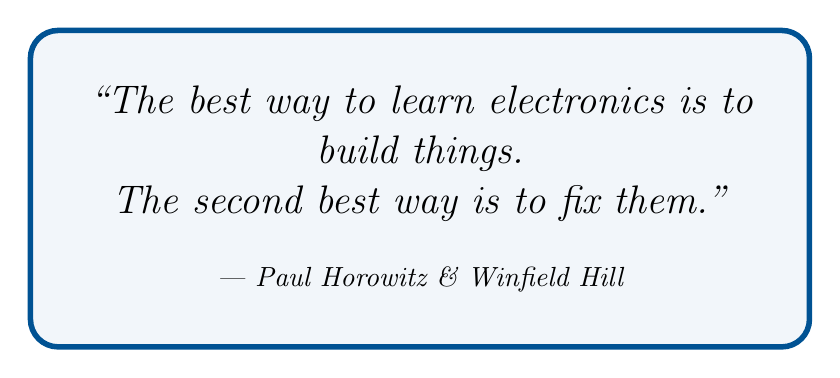
\begin{tikzpicture}
    \node[draw=chaptercolor, line width=2pt, rounded corners=10pt, 
          inner sep=20pt, fill=chaptercolor!5] {
        \begin{minipage}{0.7\textwidth}
            \centering
            \Large\itshape
            ``The best way to learn electronics is to build things.\\
            The second best way is to fix them.''\\[1em]
            \normalsize
            --- Paul Horowitz \& Winfield Hill
        \end{minipage}
    };
\end{tikzpicture}
\end{center}

\vspace*{\fill}

\end{document}
